%% SagarVaani — IEEE CONFERENCE paper (target: IEEE CONECCT 2027)
%% Framing: design + honest status. Sources: ../../raw_materials/ ; see guidelines.md.
%% Every empirical number traces to ../../raw_materials/experimental_log.md.
\documentclass[conference]{IEEEtran}
\IEEEoverridecommandlockouts
\usepackage{cite}
\usepackage{amsmath,amssymb,amsfonts}
\usepackage{graphicx}
\usepackage{xcolor}
\usepackage{booktabs}
\usepackage{array}
\usepackage{url}
\usepackage{tikz}
\usetikzlibrary{arrows.meta,positioning,shapes.geometric,fit,backgrounds}
\usepackage[hidelinks]{hyperref}

\newcommand{\NE}{\textsc{not\_evaluable}}
\newcommand{\PASS}{\textsc{pass}}
\newcommand{\BLOCK}{\textsc{block}}

% compact TikZ styles
\tikzset{
  blk/.style={draw, rounded corners=2pt, align=center, font=\scriptsize,
              inner sep=2.5pt, minimum height=5mm, fill=blue!5},
  dec/.style={draw, diamond, aspect=2, align=center, font=\scriptsize,
              inner sep=1pt, fill=orange!12},
  store/.style={draw, align=center, font=\scriptsize, inner sep=2.5pt, fill=gray!10},
  fl/.style={-{Latex[length=1.6mm]}, thick},
}

\begin{document}

\title{SagarVaani: Fail-Closed Evidence Gating and Bounded Recovery\\ for Marine and Coastal Advisories}

\author{
\IEEEauthorblockN{Syed Amaan}
\IEEEauthorblockA{\textit{Dayananda Sagar University}\\
Bengaluru, India\\
syedamaan1610@gmail.com}
\and
\IEEEauthorblockN{Mallikarjuna D M}
\IEEEauthorblockA{\textit{Dayananda Sagar University}\\
Bengaluru, India\\
dmmallikarjuna52@gmail.com}
}

\maketitle

\begin{abstract}
Marine advisories for small-scale fishers are assembled from heterogeneous, fallible data sources. A generative, agent-based advisory can remain fluent and confident when the underlying evidence is missing, stale, or mislocated, converting a data failure into an apparent assurance of safety, since in a safety setting the absence of a warning is itself a message. Known agent-orchestration controls are score-based: they measure how far agents agree, not whether a mandatory safety check could be evaluated at all. We present SagarVaani, a fail-closed, evidence-gated release interlock above a multi-agent acquisition layer. Each mandatory release check yields one of \PASS{}, \BLOCK{}, or \NE{}, where \NE{} encodes an unavailable input and can never contribute to release; the verdict follows a fixed, model-independent rule, and release occurs only on an affirmative \PASS{}. Evidence-gap recovery is confined to a closed list of actions within a finite budget, terminated when a fingerprint of unresolved gaps recurs, ending in auditable abstention rather than a synthesised advisory. We implement the architecture as a self-contained module and evaluate it with twelve deterministic experiments that reproduce the specified behaviour---affirmative-\PASS{} release, \BLOCK{}/\NE{} withholding with \BLOCK{} precedence, repair of an addressable gap within budget, an early stop on a recurring gap fingerprint, rejection of an out-of-list recovery action, and refusal of a release without \PASS{}---with the full backend suite passing 85 of 85 tests. We report behavioural correctness on reference inputs, not a field study, and claim no measured reduction in real-world risk.
\end{abstract}

\begin{IEEEkeywords}
fail-closed systems, evidence gating, abstention, multi-agent systems, decision support, marine safety, trustworthy AI
\end{IEEEkeywords}

\section{Introduction}
Persons who go to sea, including small-scale fishers, decide whether a trip is safe using forecasts of wave height, wind, currents, and related conditions. Such information is published by several agencies in differing formats, units, update cycles, and spatial resolutions, and is often not in a form a fisher can readily use. Conversational systems built on large language models and cooperating software agents have been proposed to retrieve this data, reason across it, and present the result in natural language~\cite{wang2024survey,sun2025llm,guo2024multiagent}.

A first difficulty is that such systems are generative. An advisory may be fluent and confident while resting on evidence that is missing, stale, of the wrong unit, outside a physically possible range, or drawn from a point or time other than the one asked about; large language models are known to produce fluent but unsupported output~\cite{ji2023hallucination}. In a safety setting the absence of a warning is itself a message: a user who receives no warning may infer that conditions are acceptable. A system that, when evidence is missing, silently emits a best-effort advisory therefore converts a data failure into an apparent assurance of safety~\cite{varshney2017safety}.

A second difficulty is that known approaches to controlling cooperating agents rely on scores. Agents report a confidence, agreement among agents is measured, a score is compared with a threshold, and the result is accepted or the task is repeated~\cite{sun2025llm,guo2024multiagent}. Such mechanisms assess \emph{how much} the agents agree; they do not establish that a check required before a safety advisory may issue was capable of being made at all. A check whose input is unavailable---for example whether an official storm warning is in force when no authoritative warning feed is connected---produces no score and is, in a score-based system, either omitted or treated as satisfied. Abstention frameworks reject on model confidence or cost~\cite{hendrickx2024reject,angelopoulos2023conformal}, and uncertainty-aware methods quantify predictive uncertainty~\cite{gawlikowski2023uncertainty,hullermeier2021aleatoric}; neither provides a primitive for ``a required input is unavailable, therefore withhold.''

We present \textbf{SagarVaani}, a release-control architecture in which release of a safety advisory is conditioned on affirmative satisfaction of every mandatory check, a check that cannot be evaluated is represented as such and prevents release, evidence-gap repair is confined to a closed set of sanctioned actions within a finite budget and terminated when no progress is made, and a model component cannot alter the release determination. We implement the architecture as a self-contained module and evaluate its behaviour with deterministic experiments (Sec.~\ref{sec:eval}); we report behavioural correctness on reference inputs, not a field study, and claim no measured reduction in real-world risk and no accuracy comparison against prior systems.

\noindent\textbf{Contributions.}
\begin{enumerate}
  \item A three-valued release policy (\PASS{}/\BLOCK{}/\NE{}) with a fixed, model-independent derivation in which \NE{} encodes input unavailability and prevents release (Sec.~\ref{sec:method}).
  \item A deterministic release interlock decoupled from the agents and from any learned or language-model selector, which may propose recovery but never decide the verdict.
  \item Bounded, closed-list recovery with gap fingerprinting for no-progress termination under a finite budget and deadline, ending in auditable abstention rather than a synthesised advisory.
  \item A guarded state machine and a checksummed audit store, implemented as a self-contained module (Sec.~\ref{sec:impl}) and evaluated by twelve deterministic experiments; the full backend suite passes 85 tests (Sec.~\ref{sec:eval}).
\end{enumerate}

\section{Related Work}
\textbf{Multi-agent (LLM) decision-making.} Surveys of LLM-based autonomous and multi-agent systems describe decomposition of a query among cooperating agents, parallel execution, and decision-making by cooperation, communication, and consensus~\cite{wang2024survey,guo2024multiagent}. Our base reference, Sun \emph{et al.}~\cite{sun2025llm}, surveys single- and multi-agent decision-making and highlights that multi-agent coordination can amplify error-propagation and provenance risks; its contribution is a map of how agents reach decisions, and its stated limitation is that it is a survey without a release-control mechanism. SagarVaani differs in locus: it deliberately \emph{removes} the release decision from the agents---a deterministic policy decides, and the agents only supply evidence.

\textbf{Abstention, selective prediction, and uncertainty.} The reject option lets a model abstain when confidence is low or the expected cost of answering is high~\cite{hendrickx2024reject}; conformal prediction calibrates abstention thresholds with coverage guarantees~\cite{angelopoulos2023conformal}; uncertainty surveys separate reducible (model) from irreducible (data) uncertainty~\cite{gawlikowski2023uncertainty,hullermeier2021aleatoric}. These abstain on a property of the \emph{model's} output. SagarVaani's \NE{} abstains on a property of the \emph{evidence}: whether the input a mandatory check requires was obtainable at all, independent of any confidence score.

\textbf{Trustworthy and safety-critical AI.} Work on the safety of machine learning in cyber-physical and decision systems argues for fail-safe behaviour~\cite{varshney2017safety}, and explainability research stresses auditable, inspectable decisions~\cite{arrieta2020xai,ali2023xai}. SagarVaani operationalises these as a deterministic interlock plus an audit store of check outcomes, recovery steps, and artefact checksums, so that a released or withheld advisory can be examined after the event.

\section{System Model and Methodology}
\label{sec:method}
\textbf{Overview.} SagarVaani is organised as a guarded state machine (Fig.~\ref{fig:arch}). A query arrives through a web, voice, or low-bandwidth channel; an interpreter extracts intent, location, and language; an orchestrator drives a planner that decomposes the query into a typed task graph; acquisition agents retrieve evidence concurrently; an evidence validator applies rule checks; and a release policy derives a verdict. The \texttt{released} state is reachable only from the \texttt{safety-gate-check} state and only on a \PASS{} verdict; every transition is recorded.

\textbf{Evidence records.} Each retrieved item is normalised to a record comprising a parameter, value, unit, location, source and product identifiers, one or more time attributes (observation, issue/model-run, forecast-valid, retrieval), a \emph{data mode} (live-forecast, live-observation, historical-replay, test-fixture, not-available), quality flags, and a reference to the stored raw artefact. The data mode prevents a replayed or fixture value from being presented as live; a synthetic value is never substituted for a missing one.

\textbf{Validator.} The validator applies rule checks---structure, units, physical range, freshness, temporal relevance, spatial coverage, evidence presence, attribution, artefact existence, and value consistency---and emits a set of evidence gaps, each with a code and a flag indicating whether it is addressable by a recovery action.

\textbf{Three-valued release policy.} The policy evaluates a set of mandatory checks $\{c_1,\dots,c_n\}$, each returning an outcome $o(c_i)\in\{\PASS,\BLOCK,\NE\}$. \PASS{} means the check was evaluated and satisfied; \BLOCK{} means it was evaluated and not satisfied; \NE{} means it could not be evaluated because a required input is unavailable (e.g.\ an official warning feed, protected-area geometry, or an expert-reviewed vessel threshold that is not integrated). The overall verdict is
\begin{equation}
V=\begin{cases}
\BLOCK, & \exists\, c_i:\,o(c_i)=\BLOCK,\\[1pt]
\NE, & \text{else if } \exists\, c_i:\,o(c_i)=\NE,\\[1pt]
\PASS, & \text{else } \forall\, c_i:\,o(c_i)=\PASS.
\end{cases}
\label{eq:verdict}
\end{equation}
Two consequences follow: a check that cannot be evaluated can never contribute to a release, and adding a mandatory check can only make release harder. The policy is deterministic and takes no language-model output as an input to~\eqref{eq:verdict}.

\textbf{Bounded recovery.} When $V\neq\PASS$ and an addressable gap exists, a recovery controller runs in cycles. At cycle $k$ it computes a fingerprint of the unresolved gap set $G_k$,
\begin{equation}
\phi_k=\mathcal{H}\!\left(\mathrm{canon}(G_k)\right),
\label{eq:fp}
\end{equation}
where $\mathrm{canon}(\cdot)$ is a canonical serialisation of the gap codes and $\mathcal{H}$ is SHA-256. A selector then proposes an action from a closed list $A=\{$retry-with-backoff, expand-radius, extend-window, switch-provider, load-historical-analogue, request-clarification, abstain$\}$; a proposal $a\notin A$ is rejected and rule-based selection is used instead. Recovery terminates (Fig.~\ref{fig:flow}) when
\begin{equation}
\phi_k\in\{\phi_0,\dots,\phi_{k-1}\}\ \lor\ k\ge B\ \lor\ t>\tau,
\label{eq:stop}
\end{equation}
with budget $B{=}2$ and deadline $\tau$; the first disjunct is the no-progress condition. The selector has no write path to the evidence, the checks, or the verdict, so a model component cannot cause release.

\textbf{Audit store.} For each run the system records the query and verdict, each task's status and duration, each artefact's path/size/SHA-256 checksum, each evidence record, each state transition, each recovery cycle (selector, action, gap code, outcome), and each policy-check outcome---so a released or withheld advisory can later be examined.

\begin{figure}[t]
\centering
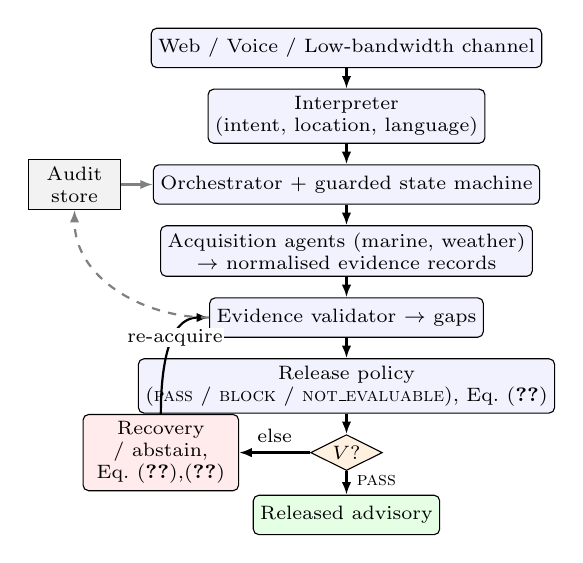
\begin{tikzpicture}[node distance=2.6mm and 4mm]
\node[blk] (chan) {Web / Voice / Low-bandwidth channel};
\node[blk, below=of chan] (intp) {Interpreter\\(intent, location, language)};
\node[blk, below=of intp] (orch) {Orchestrator + guarded state machine};
\node[blk, below=of orch] (acq) {Acquisition agents (marine, weather)\\$\rightarrow$ normalised evidence records};
\node[blk, below=of acq] (val) {Evidence validator $\rightarrow$ gaps};
\node[blk, below=of val] (pol) {Release policy\\(\PASS{} / \BLOCK{} / \NE{}), Eq.~\eqref{eq:verdict}};
\node[dec, below=2.6mm of pol] (dec) {$V$?};
\node[blk, below=3mm of dec, fill=green!10] (rel) {Released advisory};
\node[blk, left=9mm of dec, fill=red!8, text width=18mm] (abs) {Recovery / abstain, Eq.~\eqref{eq:fp},\eqref{eq:stop}};
\node[store, left=4mm of orch, text width=10mm] (aud) {Audit\\store};
\foreach \a/\b in {chan/intp,intp/orch,orch/acq,acq/val,val/pol,pol/dec}{\draw[fl] (\a)--(\b);}
\draw[fl] (dec) -- node[right,font=\scriptsize,pos=0.4]{\PASS} (rel);
\draw[fl] (dec) -- node[above,font=\scriptsize]{else} (abs);
\draw[fl] (abs.north) to[out=90,in=180] node[font=\scriptsize,fill=white,inner sep=0.5pt,pos=0.62]{re-acquire} (val.west);
\draw[fl,gray] (aud) -- (orch);
\draw[fl,gray,dashed] (val.west) to[out=180,in=-90] (aud);
\end{tikzpicture}
\caption{Fail-closed, evidence-gated release architecture. The \texttt{released} state is reachable only on an affirmative \PASS{}; otherwise the system recovers within bounds or abstains, and the audit store records every step.}
\label{fig:arch}
\end{figure}

\begin{figure}[t]
\centering
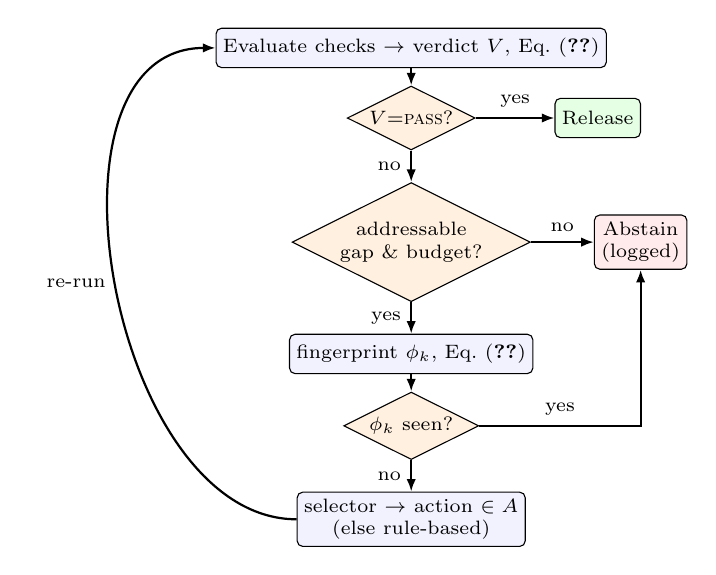
\begin{tikzpicture}[node distance=2.2mm and 4mm]
\node[blk] (v) {Evaluate checks $\to$ verdict $V$, Eq.~\eqref{eq:verdict}};
\node[dec, below=of v] (p) {$V{=}\PASS$?};
\node[blk, right=10mm of p, fill=green!10] (rel) {Release};
\node[dec, below=4mm of p] (g) {addressable\\gap \& budget?};
\node[blk, right=8mm of g, fill=red!8] (ab) {Abstain\\(logged)};
\node[blk, below=4mm of g] (f) {fingerprint $\phi_k$, Eq.~\eqref{eq:fp}};
\node[dec, below=of f] (np) {$\phi_k$ seen?};
\node[blk, below=4mm of np] (sel) {selector $\to$ action $\in A$\\(else rule-based)};
\draw[fl] (v)--(p);
\draw[fl] (p)-- node[above,font=\scriptsize]{yes}(rel);
\draw[fl] (p)-- node[left,font=\scriptsize]{no}(g);
\draw[fl] (g)-- node[above,font=\scriptsize]{no}(ab);
\draw[fl] (g)-- node[left,font=\scriptsize]{yes}(f);
\draw[fl] (f)--(np);
\draw[fl] (np)-| node[above,font=\scriptsize,pos=0.25]{yes}(ab);
\draw[fl] (np)-- node[left,font=\scriptsize]{no}(sel);
\draw[fl] (sel.west) to[out=180,in=180] node[left,font=\scriptsize]{re-run}(v.west);
\end{tikzpicture}
\caption{Three-valued release determination and bounded allow-list recovery. Termination follows Eq.~\eqref{eq:stop}; the exit without a \PASS{} verdict is abstention, never a synthesised advisory.}
\label{fig:flow}
\end{figure}

\section{Implementation}
\label{sec:impl}
The release architecture is implemented as a self-contained Python module (\texttt{backend/release/}, ${\approx}820$ lines, standard library only, deterministic). Its seven components (Table~\ref{tab:status}) are: an evidence model with the data-mode enumeration; a rule-based validator that emits coded gaps; the three-valued release policy of~\eqref{eq:verdict}; the guarded state machine with the transition table of Sec.~\ref{sec:method}; the bounded recovery controller implementing the fingerprint of~\eqref{eq:fp} and the termination rule of~\eqref{eq:stop}; the checksummed audit store; and an engine that orchestrates them and enters the \texttt{released} state only on an affirmative \PASS{}.

The module sits above the ``ORCA'' acquisition prototype (FastAPI backend, Next.js dashboard; ${\approx}8.3$k lines of backend Python), which supplies normalised evidence---wave and wind as Open-Meteo model forecasts, with currents, fishing zones, and ocean-colour values as archived or static reference data, each labelled live or non-live. The three mandatory-check inputs---an official warning feed, protected-area geometry, and expert-reviewed vessel thresholds---are supplied as configurable reference inputs; when an input is absent the corresponding check returns \NE{}, so a \PASS{} is reachable only when all three are provided.

\begin{table}[t]
\caption{Implemented components of the release module (\texttt{backend/release/})}
\label{tab:status}
\centering
\footnotesize
\begin{tabular}{@{}>{\raggedright\arraybackslash}p{5.5cm}@{\ }r@{}}
\toprule
\textbf{Component} & \textbf{Lines} \\
\midrule
Evidence model + data modes & 116 \\
Rule-based evidence validator & 196 \\
Three-valued release policy (Eq.~\ref{eq:verdict}) & 138 \\
Guarded state machine (transition table) & 56 \\
Bounded recovery + fingerprint (Eq.~\ref{eq:fp},\,\ref{eq:stop}) & 128 \\
Checksummed audit store & 68 \\
Release engine (orchestrator) & 118 \\
\midrule
\textbf{Release module core} & \textbf{820} \\
\bottomrule
\end{tabular}
\end{table}

\section{Experiments and Evaluation}
\label{sec:eval}
\textbf{Setup.} All results are produced by executing the implemented module at a fixed commit, Python 3.13.6, offline (no network, API keys, or paid endpoints), and are reproducible with \texttt{python -m release.experiments} and \texttt{python -m pytest}.

\textbf{Behavioural experiments.} Table~\ref{tab:exp} lists twelve deterministic experiments, each targeting a specified property of the architecture; every one produced the expected outcome. An all-satisfied context releases on \PASS{}; an active official warning, a wave above the vessel limit, or a protected-area intersection yields \BLOCK{} and withholds; an unavailable warning feed yields \NE{} and the system abstains; \BLOCK{} takes precedence over \NE{}. An addressable gap (missing core evidence) is repaired by a sanctioned action in a single recovery cycle and releases; the cycle budget ($B{=}2$) is exhausted after two cycles, while a recurring gap fingerprint stops recovery at the first cycle---before the budget---and a deadline likewise stops it. An out-of-list recovery proposal from a model selector is rejected and a rule-based action is logged in its place, and an attempt to reach the \texttt{released} state without a \PASS{} verdict is refused by the state machine. A successful run yields a complete, checksummed audit record (six transitions, four check records, two checksummed artefacts).

\begin{table}[t]
\caption{Release-architecture experiments and observed outcomes}
\label{tab:exp}
\centering
\footnotesize
\begin{tabular}{@{}>{\raggedright\arraybackslash}p{4.7cm}@{\ }>{\raggedright\arraybackslash}p{3.0cm}@{}}
\toprule
\textbf{Experiment} & \textbf{Observed outcome} \\
\midrule
All mandatory checks pass & \PASS{} $\to$ released \\
Active official warning & \BLOCK{} $\to$ blocked \\
Wave exceeds vessel limit & \BLOCK{} \\
Protected-area intersection & \BLOCK{} \\
Unavailable warning feed & \NE{} $\to$ abstained \\
\BLOCK{} with \NE{} present & \BLOCK{} (precedence) \\
Addressable gap repaired & succeeded, 1 cycle $\to$ released \\
Recovery budget exhausted & abstain at 2 cycles \\
Recurring gap fingerprint & no-progress at cycle 1 \\
Recovery deadline exceeded & abstain \\
Out-of-list recovery proposal & rejected; rule-based used \\
Release without \PASS{} & refused by state machine \\
\bottomrule
\end{tabular}
\end{table}

\textbf{Test suite.} The full backend suite passes \textbf{85 of 85 tests}---the 62 prototype tests plus 23 new tests that assert the experiments above together with the validator's detection of stale, malformed, unit-mismatched, out-of-range, and inconsistent evidence.

\section{Limitations and Threats to Validity}
\textbf{Construct validity.} The evaluation is behavioural and offline on deterministic fixtures: it establishes that the mechanisms behave as specified, not that real-world accidents are reduced. The three mandatory-check inputs are configurable reference inputs rather than live official feeds; with live feeds the same \NE{} logic applies whenever a feed is unavailable. \textbf{Internal validity.} The tests assert specified outcomes on constructed contexts, not emergent behaviour on operational traffic. \textbf{External validity.} The acquisition prototype is a single-region (Karnataka coast) pilot in which wave and wind are model forecasts and several layers are static reference data, not live INCOIS/IMD/ISRO feeds; transfer is not demonstrated, and we run no accuracy comparison against another system. \textbf{Independence.} The novelty positioning relative to prior patents and preprints is the authors' own assessment and has not been independently validated here.

\section{Conclusion and Future Work}
We presented and implemented SagarVaani, a fail-closed, evidence-gated release interlock that conditions a marine advisory on affirmative satisfaction of every mandatory check, represents an unevaluable check as a distinct \NE{} outcome that prevents release, confines recovery to a closed list bounded by a budget and a gap fingerprint, and abstains with an audit record rather than synthesising an unsupported advisory. Twelve deterministic experiments reproduce the specified behaviour and the full backend suite passes 85 tests. Future work is to integrate live official warning, protected-area, and vessel-limit feeds in place of the reference inputs, to deploy on the coast, and to run a field evaluation under injected live-source failures, measuring the rate of unsupported advisories against score-based baselines.

\bibliographystyle{IEEEtran}
\bibliography{references}

\end{document}
